\documentclass[11pt, oneside]{article}   	% use "amsart" instead of "article" for AMSLaTeX format
\usepackage{geometry}                		% See geometry.pdf to learn the layout options. There are lots.
\geometry{letterpaper}                   		% ... or a4paper or a5paper or ... 
%\geometry{landscape}                		% Activate for for rotated page geometry
%\usepackage[parfill]{parskip}    		% Activate to begin paragraphs with an empty line rather than an indent
\usepackage{graphicx}				% Use pdf, png, jpg, or eps§ with pdflatex; use eps in DVI mode
								% TeX will automatically convert eps --> pdf in pdflatex		
\usepackage{amssymb}
\usepackage{amsmath}
\usepackage{parskip}
\usepackage{color}
\usepackage{hyperref}

\title{Exponential distribution}
%\author{The Author}
\date{}							% Activate to display a given date or no date

\graphicspath{{/Users/telliott_admin/Dropbox/Tex/png/}}
% \begin{center} 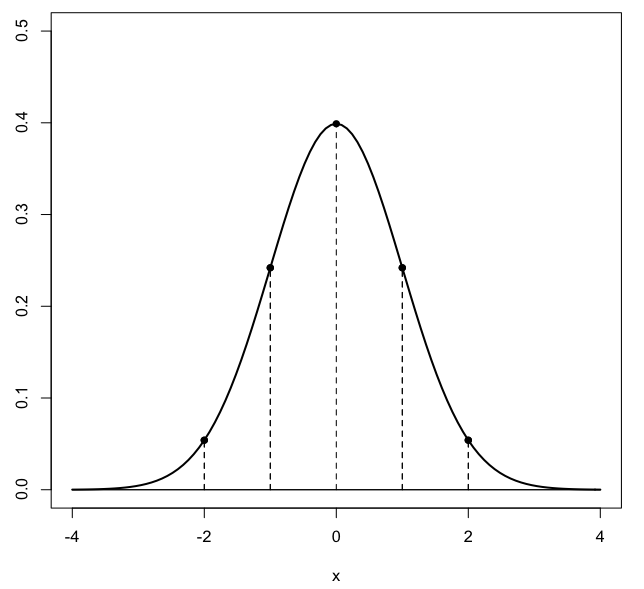
\includegraphics [scale=0.4] {gauss3.png} \end{center}

\begin{document}
\maketitle
\Large
Back in calculus, we saw the exponential function, which applies to compound interest or exponential growth.  

Suppose we have an amount or count of "stuff" $N$ (money or rabbits or radioactive phosphorus atoms).  It isn't necessary for $N$ to be an integer.

Now, suppose that $N$ changes by an amount $\Delta N$ during a short time interval $\Delta t$.  If the rate of change $\Delta N/\Delta t$ is \emph{proportional} to the amount of stuff present 
\[ \frac{\Delta N}{\Delta t} = k N \]
Then, in the limit as $\Delta t \rightarrow 0$
\[ = \frac{dN}{dt} = k N \]
Rearrange
\[ \frac{dN}{N} = k \ dt \]
Integrate
\[ \log N - \log N_0 =  kt \]
\[ \log \ \frac{N}{N_0} =  kt \]
Exponentiate:
\[ \frac{N}{N_0} = e^{kt} \]
\[ N = N_0 e^{kt} \]

The same equation also applies to exponential loss (like radioactive decay).  Just add a minus sign in front of the constant of proportionality.
\[ N = N_0 e^{-kt} \]

Let's stop for a minute and go back to distributions from standard probability theory:   we talk about probability density function $p(x)$ and say that the probability that the random variable $x$ lies in an interval $[a,b]$ is
\[ P(a < x < b) = \int_a^b p(x) \ dx \]

Furthermore, the cumulative density function or cdf is usually called $F(x)$ and is
\[ F(x) = \int p(x) \ dx \]
\[ P(a < x < b) = F(x) \ \bigg |_a^b \]
\[ P( x < b) = F(x) \ \bigg |_0^b = F(b) \]

Suppose we just accept for a moment that the probability density function (pdf) for the negative exponential has this form
\[ p(t) = \lambda e^{-\lambda t} \ \ \ (t \ge 0) \]
Use of $\lambda$ for the constant is traditional.  $\lambda$ is defined to be the the mean number of events per unit time, and the probability that a random event occurs during the interval $[t_1,t_2]$ is the integral
\[ \int_{t_1}^{t_2} \ p(t) \ dt \]

The cumulative distribution function (cdf) corresponding to this pdf is the above integral:
\[ cdf(x) = \int \lambda e^{-\lambda t} \ dt \]
\[ =  - e^{-\lambda t} + C \]
The constant of integration is just $1$:
\[ cdf(t) = 1 - e^{-\lambda t} \]

It is determined from the boundary conditions.  With the lower bound at zero, then as $t$ gets very large the total probability must go to $1$.
\[ cdf(t) = 1 - e^{-\lambda t} \]
This also works for the other boundary condition, namely $cdf(0) = 0$.

The probability that an event has not yet happened (happens after this time) is $1$ minus this or
\[ P(x > t) = e^{-\lambda t}  \]

We can use this distribution to model the time that passes until a randomly occurring event.

To determine the probability that the event happens after time $t$ we integrate $p(x)$, or just evaluate the cdf at the bounds:
\[ \int_t^{\infty} \lambda e^{-\lambda x} \ dx \]
\[ = 1 - e^{-\lambda x}  \ \bigg |_t^{\infty} \]

The integral is just the cdf evaluated at the two bounds.  To deal with infinity first solve for $\int_t^T $ (with $T > t$ and very large):
\[ p(x > t) = 1 - e^{-\lambda x} \ \bigg |_t^T = -  e^{-\lambda T} +  e^{-\lambda t} \]

The first term becomes zero as $T \rightarrow \infty$ so
\[ p(x > t) = e^{-\lambda t} \]
The probability that the event will happen after $t = 0$ is equal to $1$, as expected.

If $\lambda$ is the number of events in a unit interval (the mean number of events per unit time), and $\theta$ is the mean waiting time until the first event, then
\[ \lambda = \frac{1}{\theta} \]

The expected number of events in a short time $\Delta t$ is just $\lambda \Delta t$.

$\circ$ Suppose the mean number of customers arriving at a bank in a 1-hour interval is 10. The average (waiting) time between customer arrivals is 1/10 of an hour, or 6 minutes.  Preferring to measure time in hours, we set
\[ \lambda = 10 \]
(called a Poisson rate) and use the cdf
\[ p(x > t) = e^{-\lambda t} = e^{- (10) \cdot t} \]

The probability of a wait time longer than the mean of $10$ minutes is
\[ p(x > 1/10) = e^{-\lambda t} = e^{-1} \] 
\[ = \frac{1}{e} = 0.37 \]
and the probability of a wait longer than $30$ minutes is $1/e^3 \approx 0.05$.

\subsection*{discrete case:  geometric distribution}

David Morin:
\begin{quote}\color{blue}Consider a process where we roll a hypothetical 10-sided die once every second. So time is discretized into 1-second intervals.

If the die shows a 1, we'll consider that a success. The other nine numbers represent failure.
\color{black}\end{quote}
We expect to have one success every $10$ rolls, and expect to wait 10 seconds for the next success, on the average.

In general, if the probability of success on each trial is $p$, the average waiting time is $1/p$.  With $n$ trials we expect that $pn$ of them will be a success, the average wait time is $n/pn = 1/p$.

What is the probability that we have to wait through $k$ trials or intervals for a success?  We must have failure on the first $k-1$ iterations followed by a single success so
\[ P = (1-p)^{k-1} \ p \]
This is called the geometric distribution, because the change in probability when going from one iteration to the next is obtained by multiplying by a constant ratio $1-p$.

\begin{quote}\color{blue}If p = 1/ 10, the distribution is maximum at k = 1 and falls off from that value. Even though k = 10 is the average waiting time, the probability of the waiting time being exactly k = 10 is only $P(10) = (0.9)^9 (0.1) \approx 0.04$.

\begin{center} 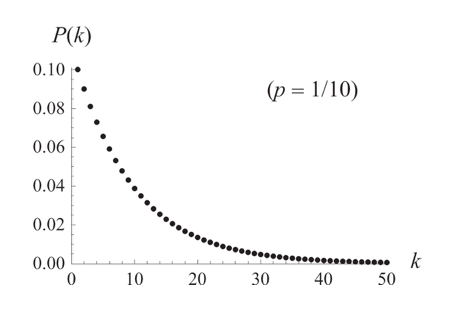
\includegraphics [scale=0.4] {exp_distr.png} \end{center}

If p is large (close to 1), the plot of P(k) starts high (at p, which is close to 1) and then falls off quickly, because the factor (1 - p) is close to 0. On the other hand, if p is small (close to 0), the plot of P(k) starts low (at p, which is close to 0) and then falls off slowly, because the factor (1 - p) is close to 1.
\end{quote}\color{black}

\subsection*{derivation of continuous case}
Consider a process in which random events occur with an average rate $\lambda$.

Chop up that time interval into many small sub-intervals $\Delta t$.  The probability that an event occurs during a time $\Delta t$ is (approximately) equal to $\lambda \Delta t$.  

(There is a small chance that two or more events will occur in the interval.  But if we make $\Delta t$ small enough, this will be negligible).

The chance that no event occurs is the complement, $1 - \lambda \Delta t$.

Now, we write $q(t)$ for the probability that \emph{no event occurs before} $t$.  Then, the probability that no event occurs before $t + \Delta t$ is the product of these two probabilities, namely
\[ q(t + \Delta t) = q(t)(1 - \lambda \Delta t) \]

Rearranging
\[ q(t + \Delta t) - q(t) = - \lambda q(t) \Delta t \]
\[ \frac{q(t + \Delta t) - q(t)}{\Delta t} = - \lambda q(t) \]
In the limit as $\Delta t \rightarrow 0$ the left-hand side becomes the derivative:
\[ q'(t) = -  \lambda q(t) \]

The negative exponential is a solution to this differential equation:
\[ q(t) = e^{-\lambda t} + C \]

Define $F(t)$ as the complement, the probability that an event \emph{does} happen before time $t$:
\[ F(t) = 1 - e^{-\lambda t} - C \]
Evaluation for the initial condition $F(0) = 0$ shows that $C = 0$ so:
\[ F(t) = 1 - e^{-\lambda t} \]

This function $F(t)$ is the cumulative density function, or cdf.  The pdf is the derivative of the cdf:
\[ p(t) = \lambda e^{-\lambda t} \]

\subsection*{memoryless property}

For any time $t$, the probability that an event has not occurred is
\[ p(x > t) = e^{-\lambda t}  \]

At some later time $t + \Delta t$, the probability is
\[ p(x > t + \Delta t) = e^{-\lambda (t + \Delta t)}  \]

We ask, what is the ratio 
\[ \frac{ p(x > t + \Delta t) }{ p(x > t) } =  \frac{e^{-\lambda (t + \Delta t)} } {  e^{-\lambda t}} \]
\[ = e^{-\lambda \Delta t} \]

This ratio is independent of the time $t$.  The fractional change in probability after a change in time $\Delta t$ does not depend on where we are on the curve.

Another way of stating this is to say that if we change the time scale of the distribution by choosing some time $t$ as zero-time, and then divide by the probability that an event did happen before that, we obtain the same distribution function back again.

Here is another proof I found on the web.

$\bullet$ A variable $X$ with positive support is \emph{memoryless} if for all $t > 0$ and $s > 0$:
\[ P(X > s+t \ | \ X > t) = P(X > s) \]
Using the definition of conditional probability:
\[ P(X > s+t) = P(X > s) \cdot P(X > t) \]

If the two probabilities $P(X > s)$ and $P(X > t)$ are independent, then the distribution is memoryless and then $P(X > s + t)$ is as stated above.

Now, the cdf of the exponential distribution is
\[ cdf(x) = 1 - e^{-\lambda x} \]
and the probability that $X > t$ is $1$ minus this or
\[ p(X > t) = e^{-\lambda t} \]

So we have:
\[ P(X > s+t) = P(X > s) \cdot P(X > t) \]
\[ = e^{-\lambda s} \cdot e^{-\lambda t} \]
\[ = e^{-\lambda (s+t)} \]

To put it the other way around, we are looking for a cumulative distribution function with the property that 
\[ P(X > s+t) = P(X > s) \cdot P(X > t) \]
for \emph{any} $s$ and $t$ so the two probabilities on the right are independent.  The exponential has this property since:
\[ e^{-\lambda (s+t)} = e^{-\lambda s} \cdot e^{-\lambda t} \]

\subsection*{Expected values:  mean and variance}
For a continuous variable
\[ E(x) = \int x \ f(x) \ dx \]
So here we have
\[ E(t) = \int_0^{\infty} t \ \lambda e^{-\lambda t} \ dt \]

We use integration by parts.  Let
\[ u = t, \ \ \ dv = \lambda e^{-\lambda t} \ dt \]
\[ du = dt, \ \ \ v = -e^{-\lambda t} \]
\[ E(t) = t (-e^{-\lambda t}) + \int e^{-\lambda t} \ dt \]
\[ = t (-e^{-\lambda t}) - \frac{e^{-\lambda t}}{\lambda} \]

and evaluate between $0 \rightarrow \infty$ by the usual method of choosing a large $T$ and then letting $T \rightarrow \infty$.  In this case, the first term at the upper bound is a little tricky, but it will turn out to equal zero, which is clearly true for the second term.  

This leaves $(-1)$ times the above or
\[ E(t) = - t \ (-e^{-\lambda t}) + \frac{e^{-\lambda t}}{\lambda} \]
evaluated at $t = 0$, giving
\[ E(t) = \frac{1}{\lambda} \]
which makes perfect sense.  If items arrive at a rate $\lambda$, then the average time to wait is the inverse of that.

It remains to evaluate
\[ \lim_{T \rightarrow \infty}  T \ (-e^{-\lambda T}) \]
Rewrite this as a ratio:
\[ \lim_{T \rightarrow \infty}  -\frac{T}{e^{\lambda T}} \]

The limit for both numerator and denominator is $\infty$.  We may use L'Hopital's Rule.  Taking the derivatives:
\[ \lim_{T \rightarrow \infty}  -\frac{1}{\lambda e^{\lambda T}}  = 0\]

Python confirms that the exponential dominates (and having $\lambda > 1$ makes it much worse).

\begin{verbatim}
>>> def f(t,k):
...     return e**(-k*t)
... 
>>> def g(t,k):
...     return k * t * f(t,k)
... 
>>> g(10,1)
0.00045399929762484877
\end{verbatim}

As a check, let's try the second moment using integration by parts:
\[ \int_0^{\infty} t^2 \ \lambda e^{-\lambda t} \ dt \]
Let
\[ u = t^2, \ \ dv = \lambda e^{-\lambda t} \ dt \]
\[ du = 2 t \ dt, \ \ v = -e^{-\lambda t} \]
So the integral is
\[ = -t^2 e^{-\lambda t} + \ 2 \ [ \int t e^{-\lambda t} \ dt \ ] \]
\[ = -t^2 e^{-\lambda t }+ \frac{2}{\lambda} \ [  \ t \ (-e^{-\lambda t}) - \frac{e^{-\lambda t}}{\lambda} \ ]  \]
The negative exponential also dominates the square of $t$ and goes to zero as $t \rightarrow \infty$ (by two applications of L'Hopital).  Hence, we just evaluate at $t=0$ and then multiply by $-1$.
\[ = 0 + \frac{2}{\lambda} \ [  0 - \frac{1}{\lambda} \ ]  \]
The switch in sign gives:
\[ \frac{1}{\lambda^2} \]

\subsection*{Advanced results}
These results can slo be obtained by using what is called a moment-generating function.

Restating what we have:
\[ E(X^2) =  \int_0^{\infty} t^2 \ \lambda e^{-\lambda t} \ dt \]
\[ = \frac{2}{\lambda^2} \]

Assuming this result for the moment,
\[ \text{Var}(x) = E(X^2) - (E(X))^2 = \frac{1}{\lambda^2} \]

The moment generating function is
\[ \phi(t) = E[e^{tX}] = \frac{\lambda}{\lambda - t}, \ \ \ t < \lambda \]
We confirm the previous results:
\[ E(X) = \frac{d}{dt} \phi(t) \ \bigg |_{t = 0} \]
\[ = \frac{\lambda}{(\lambda - t)^2} \ \bigg |_{t = 0} = \frac{1}{\lambda} \]
and
\[ E(X^2) = \frac{d^2}{dt^2} \phi(t) \ \bigg |_{t = 0} \]
\[ = \frac{2 \lambda}{(\lambda - t)^3} \ \bigg |_{t = 0} = \frac{2}{\lambda^2} \]

\subsection*{Examples}
The exponential distribution or pdf is
\[ p(t) = \lambda e^{-\lambda t} \]
The probability of occurrence of a random event in some particular interval is the integral of the pdf between those bounds, namely the cdf simply evaluated for the same bounds
\[ cdf(t) = \int p(t) \ dt \]
\[ = 1 - e^{-\lambda t} \]

(the constant being determined by the requirement that the total be equal to $1$, but it doesn't matter since it will cancel anyway).
\[ = - e^{-\lambda t}  \ \bigg |_{t_1}^{t_2} \]
\[ = e^{-\lambda t_1} - e^{-\lambda t_2}, \ \ \ (t_1 < t_2) \]
The probability that \emph{no event occurs} in an interval $[t_1,t_2]$ is
\[ 1 - \ [ \ e^{-\lambda t_1} - e^{-\lambda t_2} \ ] \]

$\circ$ If jobs arrive every 15 seconds on average (so $\lambda = 4$ jobs per minute), what is the probability of waiting 30 seconds or less?  ($t_1 = 0, \ t_2 = 0.5$).
\[ P(T \le 0.5) = e^{-\lambda t_1} - e^{-\lambda t_2} \]
\[ = e^{0} - e^{-4 \cdot (0.5)} \]
\[ = 1 - e^{-2} = 0.865 \]

From R:
\begin{verbatim}
pexp(0.5,4)
[1] 0.8646647
\end{verbatim}

$\circ$ For the same rate, what is the maximum waiting time between two jobs with 95\% confidence?
\[ = 1 - e^{-\lambda t} = 0.95 \]
\[ 0.05 = e^{-\lambda t} \]
\[ \ln 0.05 = - \lambda t \]
\[ -3.0 = -4 \cdot t \]
\[ t = 0.75 \]
There is a 95\% probability that the time between jobs is less than 45 seconds.
\begin{verbatim}
qexp(0.95,4)
[1] 0.7489331
\end{verbatim}

$\circ$ Accidents occur with a Poisson distribution at a rate of 4 per week.  What is the probability of more than 3 accidents in one week?

The Poisson distribution is
\[ P(i) = \frac{e^{-m} m^i}{i!} \]
(which I remember as Emmii).  More common notation is
\[ P(k) = \frac{e^{-\lambda} \lambda^k}{k!} \]
So $\lambda = 4$ and
\[ e^{- \lambda} = 0.0183 \]
and
\[ P(0) = 0.183 \cdot  \frac{4^0}{0!} = 0.0183  \]
\[ P(1) = 0.183 \cdot  \frac{4^1}{1!} = 0.0737  \]
\[ P(2) = 0.183 \cdot  \frac{4^2}{2!} = 0.1465  \]
The probability is $1$ minus the sum of these, or about $0.76$.

In R, the probability of $k$ or fewer is ppois$(k, lambda=4)$:
\begin{verbatim}
> 1 - ppois(2,4)
[1] 0.7618967
\end{verbatim}

What is the probability that at least two weeks will elapse between accidents?
\[ 1 - \ [ \ e^{-\lambda t_1} - e^{-\lambda t_2} \ ] \]
\[ 1 - \ [ \ e^{-\lambda \cdot(0)} - e^{-4 \cdot (2)} \ ] \]
\[ = e^{-8} = 0.000335 \]

\begin{verbatim}
> 1 - pexp(2,4)
[1] 0.0003354626
\end{verbatim}


\end{document}  